% =============================================================================
% Lecture 07: Machine Learning Introduction
% BSAD 8310: Business Forecasting
% University of Nebraska at Omaha
% =============================================================================

\documentclass[aspectratio=169, 11pt]{beamer}

% =============================================================================
% header.tex — BSAD 8310: Business Forecasting
% University of Nebraska at Omaha
% Beamer theme: UNO-branded, clean, professional
% =============================================================================

% ----------------------------- BEAMER THEME ----------------------------------
\usetheme{default}
\useinnertheme{rectangles}

% ----------------------------- UNO COLOR PALETTE -----------------------------
\definecolor{unoblue}{HTML}{005CA9}
\definecolor{unored}{HTML}{E41C38}
\definecolor{unogray}{HTML}{525252}
\definecolor{unogreen}{HTML}{15803d}
\definecolor{unolightblue}{HTML}{E8F0FA}
\definecolor{unolightred}{HTML}{FDECEA}
\definecolor{unolightgreen}{HTML}{F0FAF4}
\definecolor{unowhite}{HTML}{FFFFFF}

% Apply UNO colors to Beamer structure
\setbeamercolor{structure}{fg=unoblue}
\setbeamercolor{palette primary}{bg=unoblue, fg=white}
\setbeamercolor{palette secondary}{bg=unoblue!80!black, fg=white}
\setbeamercolor{palette tertiary}{bg=unoblue!60!black, fg=white}
\setbeamercolor{frametitle}{bg=unoblue, fg=white}
\setbeamercolor{frametitle right}{bg=unoblue!80!black}
\setbeamercolor{title}{fg=unoblue}
\setbeamercolor{subtitle}{fg=unogray}
\setbeamercolor{author in head/foot}{bg=unoblue, fg=white}
\setbeamercolor{title in head/foot}{bg=unoblue!80, fg=white}
\setbeamercolor{date in head/foot}{bg=unoblue!60, fg=white}
\setbeamercolor{page number in head/foot}{bg=unoblue!60, fg=white}
\setbeamercolor{block title}{bg=unoblue, fg=white}
\setbeamercolor{block body}{bg=unolightblue}
\setbeamercolor{block title alerted}{bg=unored, fg=white}
\setbeamercolor{block body alerted}{bg=unolightred}
\setbeamercolor{block title example}{bg=unogreen, fg=white}
\setbeamercolor{block body example}{bg=unolightgreen}
\setbeamercolor{itemize item}{fg=unoblue}
\setbeamercolor{itemize subitem}{fg=unored}
\setbeamercolor{enumerate item}{fg=unoblue}
\setbeamercolor{enumerate subitem}{fg=unored}
\setbeamercolor{alerted text}{fg=unored}

% ----------------------------- FONTS -----------------------------------------
\usefonttheme{professionalfonts}
\usefonttheme[onlymath]{serif}       % serif math; sans-serif text
\setbeamerfont{frametitle}{size=\large, series=\bfseries}
\setbeamerfont{title}{size=\LARGE, series=\bfseries}
\setbeamerfont{subtitle}{size=\large}
\setbeamerfont{block title}{size=\normalsize, series=\bfseries}
\setbeamerfont{footline}{size=\tiny}

% ----------------------------- LAYOUT ----------------------------------------
\setbeamersize{text margin left=0.5cm, text margin right=0.5cm}
\setbeamertemplate{navigation symbols}{}   % remove navigation buttons
\setbeamertemplate{itemize items}[circle]
\setbeamertemplate{enumerate items}[default]

% Custom footline: [Course] [Title] [Page/Total]
\setbeamertemplate{footline}{%
  \leavevmode%
  \hbox{%
    \begin{beamercolorbox}[wd=.33\paperwidth, ht=2.5ex, dp=1ex, left, leftskip=4pt]
      {author in head/foot}%
      \usebeamerfont{author in head/foot}\insertshortauthor
    \end{beamercolorbox}%
    \begin{beamercolorbox}[wd=.34\paperwidth, ht=2.5ex, dp=1ex, center]
      {title in head/foot}%
      \usebeamerfont{title in head/foot}\insertshorttitle
    \end{beamercolorbox}%
    \begin{beamercolorbox}[wd=.33\paperwidth, ht=2.5ex, dp=1ex, right, rightskip=4pt]
      {date in head/foot}%
      \usebeamerfont{date in head/foot}%
      \insertframenumber{} / \inserttotalframenumber
    \end{beamercolorbox}%
  }%
  \vskip0pt%
}

% Frametitle with thin accent line
\setbeamertemplate{frametitle}{%
  \vskip0.1cm
  \insertframetitle
  \vskip0.05cm
  \color{unored}\rule{\textwidth}{0.5pt}
}

% Title page
\setbeamertemplate{title page}{%
  \vfill
  \begin{center}
    {\color{unoblue}\rule{\textwidth}{2pt}}\\[0.3cm]
    {\usebeamerfont{title}\usebeamercolor[fg]{title}\inserttitle}\\[0.2cm]
    {\usebeamerfont{subtitle}\usebeamercolor[fg]{subtitle}\insertsubtitle}\\[0.3cm]
    {\color{unored}\rule{\textwidth}{0.5pt}}\\[0.4cm]
    {\small\insertauthor}\\[0.1cm]
    {\small\insertinstitute}\\[0.1cm]
    {\small\insertdate}
  \end{center}
  \vfill
}

% ----------------------------- PACKAGES --------------------------------------

% Math
\usepackage{amsmath}
\usepackage{amssymb}
\usepackage{mathtools}
\usepackage{bm}                    % bold math symbols

% Graphics & color
\usepackage{graphicx}
\usepackage{xcolor}
\usepackage{tikz}
\usetikzlibrary{arrows.meta, positioning, shapes, fit, backgrounds, calc}
\usepackage{pgfplots}
\pgfplotsset{compat=1.18}

% Tables
\usepackage{booktabs}
\usepackage{array}
\usepackage{multirow}
\usepackage{tabularx}

% Typography
\usepackage{microtype}
\usepackage{url}
\usepackage{hyperref}
\hypersetup{colorlinks=true, linkcolor=unoblue, urlcolor=unoblue, citecolor=unogray}

% Code listings (no shell-escape required)
\usepackage{listings}
\lstset{
  language=Python,
  basicstyle=\ttfamily\footnotesize,
  keywordstyle=\color{unoblue}\bfseries,
  stringstyle=\color{unogreen},
  commentstyle=\color{unogray}\itshape,
  numberstyle=\tiny\color{unogray},
  breaklines=true,
  showstringspaces=false,
  frame=single,
  rulecolor=\color{unogray!40},
  backgroundcolor=\color{unogray!5},
  xleftmargin=0.5em,
  xrightmargin=0.5em,
}

% Bibliography
\usepackage[backend=bibtex, style=authoryear, maxcitenames=2]{biblatex}
\addbibresource{../Bibliography_base.bib}

% Colored text helpers
\usepackage{tcolorbox}
\tcbuselibrary{skins, breakable, listingsutf8}

% ----------------------------- CUSTOM ENVIRONMENTS ---------------------------

% keybox: UNO-blue background — for key results, formulas, takeaways
\newtcolorbox{keybox}{
  enhanced,
  colback=unoblue,
  colframe=unoblue!80!black,
  coltitle=white,
  coltext=white,
  fonttitle=\bfseries,
  boxrule=0pt,
  arc=3pt,
  left=4pt, right=4pt, top=3pt, bottom=3pt,
}

% definitionbox: blue left-rule with title — for formal definitions
\newtcolorbox{definitionbox}[1]{
  enhanced,
  title={#1},
  colback=unolightblue,
  colframe=unoblue,
  coltitle=unoblue,
  fonttitle=\bfseries,
  boxrule=0pt,
  leftrule=3pt,
  arc=0pt,
  left=4pt, right=4pt, top=3pt, bottom=3pt,
}

% warningbox: red-accent — for pitfalls, assumption violations, common errors
\newtcolorbox{warningbox}{
  enhanced,
  colback=unolightred,
  colframe=unored,
  coltitle=white,
  fonttitle=\bfseries,
  boxrule=0pt,
  leftrule=3pt,
  arc=0pt,
  left=4pt, right=4pt, top=3pt, bottom=3pt,
}

% examplebox: green-accent with title — for worked examples, business applications
\newtcolorbox{examplebox}[1]{
  enhanced,
  title={#1},
  colback=unolightgreen,
  colframe=unogreen,
  coltitle=unogreen,
  fonttitle=\bfseries,
  boxrule=0pt,
  leftrule=3pt,
  arc=0pt,
  left=4pt, right=4pt, top=3pt, bottom=3pt,
}

% ----------------------------- MATH SHORTCUTS --------------------------------
\newcommand{\E}{\mathbb{E}}
\newcommand{\Var}{\operatorname{Var}}
\newcommand{\Cov}{\operatorname{Cov}}
\newcommand{\Corr}{\operatorname{Corr}}
\newcommand{\MSE}{\operatorname{MSE}}
\newcommand{\RMSE}{\operatorname{RMSE}}
\newcommand{\MAE}{\operatorname{MAE}}
\newcommand{\MASE}{\operatorname{MASE}}
\newcommand{\yhat}{\hat{y}}
\newcommand{\bhat}{\hat{\beta}}
\newcommand{\eps}{\varepsilon}
\newcommand{\given}{\,|\,}

% ----------------------------- SLIDE HELPERS ---------------------------------
% Section title slide (call at start of each section)
\newcommand{\sectionslide}[2]{%
  \begin{frame}
    \vfill
    \begin{center}
      {\color{unoblue}\rule{0.6\textwidth}{2pt}}\\[0.4cm]
      {\Large\bfseries\color{unoblue} #1}\\[0.2cm]
      {\normalsize\color{unogray} #2}\\[0.4cm]
      {\color{unored}\rule{0.6\textwidth}{1pt}}
    \end{center}
    \vfill
  \end{frame}
}

% Muted text
\newcommand{\muted}[1]{{\color{unogray}#1}}

% Key term
\newcommand{\key}[1]{{\color{unoblue}\textbf{#1}}}

% Positive / negative annotations
\newcommand{\pos}[1]{{\color{unogreen}#1}}
\newcommand{\negc}[1]{{\color{unored}#1}}


% ---- Lecture metadata --------------------------------------------------------
\title{Machine Learning Introduction}
\subtitle{BSAD 8310: Business Forecasting --- Lecture 7}
\author{Department of Economics}
\institute{University of Nebraska at Omaha}
\date{Spring 2026}

% =============================================================================
\begin{document}
% =============================================================================

\begin{frame}
  \titlepage
\end{frame}

% --- Outline -----------------------------------------------------------------
\begin{frame}{Lecture 7: Outline}
  \tableofcontents
\end{frame}

% =============================================================================
\section{Why ML for Forecasting?}
% =============================================================================

\sectionslide{Why ML for Forecasting?}{%
  Classical methods are powerful --- but structured.
  What happens when the structure breaks?}

% --- Slide: Limits of classical forecasting -----------------------------------
\begin{frame}{The Limits of Classical Forecasting}
  Six lectures built a powerful toolkit. Now we stress-test its assumptions.
  \begin{columns}[T]
    \column{0.50\textwidth}
      \textbf{What we have (L01--L06):}
      \begin{itemize}\small
        \item Benchmarks and regression (L01--L02)
        \item ETS for trend + seasonality (L03)
        \item ARIMA/SARIMA for autocorrelation (L04)
        \item VAR, ARIMAX, ECM for multivariate dynamics (L05)
        \item Rigorous walk-forward evaluation (L06)
      \end{itemize}
    \column{0.46\textwidth}
      \begin{warningbox}
        {\small Classical models assume: linearity, fixed lag
        structure, Gaussian errors, known seasonality.
        When these fail, \textbf{model misspecification}
        inflates forecast error beyond what better data
        could fix.}
      \end{warningbox}
  \end{columns}
  \muted{\footnotesize\itshape
    Socratic: which assumption fails first when forecasting
    social-media-driven demand spikes for a new product?}
\end{frame}

% --- Slide: Three gaps ML fills -----------------------------------------------
\begin{frame}{Three Gaps ML Fills}
  \begin{columns}[T]
    \column{0.54\textwidth}
      {\footnotesize
      \begin{tabular}{p{2.0cm}p{2.6cm}p{2.0cm}}
        \toprule
        \textbf{Gap} & \textbf{Classical limit} & \textbf{ML remedy} \\
        \midrule
        Non-linearity  & Linear $f(x)$ assumed  & Trees, nets \\
        Many predictors & VAR fails ($p>T$)      & Regularization \\
        Interactions   & Hand-specified only     & Learned \\
        Non-Gaussian   & Normality assumed       & Distribution-free \\
        \bottomrule
      \end{tabular}
      }
    \column{0.42\textwidth}
      \begin{keybox}
        {\small ML does \textbf{not} replace ARIMA.
        It extends the toolkit for problems where:
        (1)~predictors number in the hundreds,
        (2)~relationships are non-linear, or
        (3)~structure is unknown \textit{a priori}.}
      \end{keybox}
  \end{columns}
  \muted{\footnotesize\itshape
    \parencite{Hastie2009}: the statistical learning perspective
    on non-linearity and interactions.}
\end{frame}

% --- Slide: Competition evidence ----------------------------------------------
\begin{frame}{Evidence: The M4 Competition}
  \textbf{100{,}000 time series, 61 methods} \parencite{Makridakis2020}:
  nine of the top twelve methods were \emph{hybrid} (classical + ML).
  \begin{columns}[T]
    \column{0.52\textwidth}
      {\footnotesize
      \begin{tabular}{lrc}
        \toprule
        \textbf{Method} & \textbf{Rank} & \textbf{sMAPE} \\
        \midrule
        Hybrid ES-RNN (ML + ETS)  & 1  & 11.37 \\
        Theta (classical)         & 2  & 11.37 \\
        FFORMA (ML ensemble)      & 3  & 11.57 \\
        Naive 2 (seasonal)        & 12 & 13.56 \\
        Auto ARIMA                & 14 & 13.58 \\
        \bottomrule
      \end{tabular}
      }
    \column{0.44\textwidth}
      \begin{examplebox}{Business context}
        {\small Retail, electricity, and supply-chain
        forecasting now routinely use gradient-boosted
        trees and ensemble combinations of ARIMA + ML.\\[3pt]
        But: pure ML often \emph{underperforms} naive on
        short series ($n < 100$). Context matters.}
      \end{examplebox}
  \end{columns}
\end{frame}

% =============================================================================
\section{The Bias-Variance Tradeoff}
% =============================================================================

\sectionslide{The Bias-Variance Tradeoff}{%
  Every modelling decision shifts error between bias and variance.
  This is the central tension in all of statistical learning.}

% --- Slide: Formal decomposition ----------------------------------------------
\begin{frame}{MSE Decomposition}
  \begin{definitionbox}{Bias-Variance Decomposition \parencite{Hastie2009}}
    {\small
    Let $\hat{f}$ be an estimated model and $f$ the true function.
    At a new point $x_0$:
    \[
      \MSE(\hat{f}(x_0))
      = \bigl(\operatorname{Bias}[\hat{f}(x_0)]\bigr)^2
        + \Var[\hat{f}(x_0)] + \sigma^2
    \]
    $\sigma^2$ = irreducible noise (no model eliminates this).}
  \end{definitionbox}
  \begin{columns}[T]
    \column{0.54\textwidth}
      \begin{itemize}\small
        \item \textbf{Bias\textsuperscript{2}}: systematic error from
              wrong model class (underfitting)
        \item \textbf{Variance}: sensitivity to particular training
              sample (overfitting)
        \item \textbf{$\sigma^2$}: irreducible --- better models cannot
              reduce this, only better data can
      \end{itemize}
    \column{0.42\textwidth}
      \muted{\footnotesize
        $\hat{f}$: estimated model.
        $f$: true unknown function.
        $x_0$: feature vector at new observation.
        $\sigma^2 = \Var[\varepsilon]$ where
        $\varepsilon$ is the noise term.}
  \end{columns}
\end{frame}

% --- Slide: Bias and variance in plain language -------------------------------
\begin{frame}{Bias and Variance in Plain Language}
  \textbf{Both extremes hurt.}
  \begin{columns}[T]
    \column{0.50\textwidth}
      \begin{examplebox}{High bias --- underfitting}
        {\small AR(1) fit to a threshold non-linear series:
        the model systematically underestimates peaks
        and overestimates troughs every cycle.\\[3pt]
        Low variance: refit on any subsample and the
        errors look the same.}
      \end{examplebox}
    \column{0.46\textwidth}
      \begin{warningbox}
        {\small High variance --- overfitting:\\[2pt]
        Degree-15 polynomial fits every wiggle in the
        training set. Train RMSE $\approx 0.02$.
        Test RMSE $\approx 8\times$ train RMSE.\\[3pt]
        Small change in training data $\Rightarrow$
        large change in $\hat{f}$.}
      \end{warningbox}
  \end{columns}
  \vspace{0.1cm}
  Reducing bias \emph{typically} increases variance.
  We control the tradeoff via \textbf{model complexity} and
  \textbf{regularization}.
\end{frame}

% --- Slide: The U-shaped complexity curve -------------------------------------
\begin{frame}{The Complexity Curve}
  Train error always falls with complexity. Test error has a U-shape.
  \begin{center}
  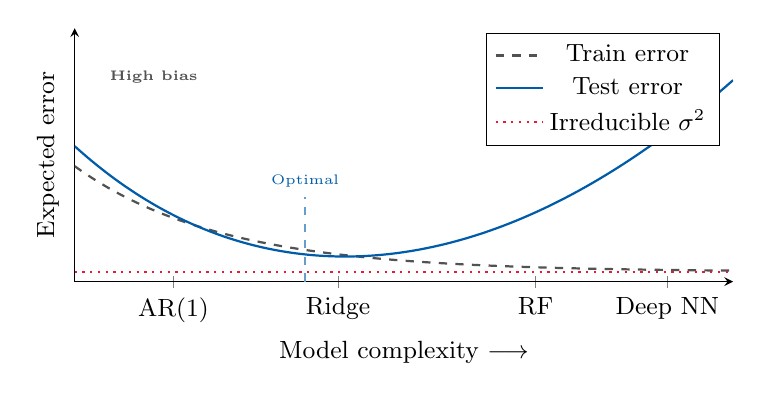
\begin{tikzpicture}
    \begin{axis}[
      width=0.82\textwidth, height=4.8cm,
      xlabel={\small Model complexity $\longrightarrow$},
      ylabel={\small Expected error},
      xmin=0, xmax=10, ymin=0, ymax=1.8,
      xtick={1.5, 4, 7, 9},
      xticklabels={AR(1), Ridge, RF, Deep NN},
      ytick=\empty,
      tick label style={font=\small},
      label style={font=\small},
      legend style={font=\small, at={(0.98,0.98)}, anchor=north east},
      axis lines=left,
      restrict y to domain=0:2,
    ]
      % Train error: monotone decreasing
      \addplot[color=unogray, thick, dashed,
               domain=0:10, samples=150]
        {0.75*exp(-0.45*x) + 0.07};
      \addlegendentry{Train error}
      % Test / validation error: U-shape
      \addplot[color=unoblue, thick,
               domain=0:10, samples=150]
        {0.5*exp(-0.40*x) + 0.07 + 0.032*(x - 3.5)^2};
      \addlegendentry{Test error}
      % Irreducible noise floor
      \addplot[color=unored, thick, dotted,
               domain=0:10, samples=2]
        {0.07};
      \addlegendentry{Irreducible $\sigma^2$}
      % Optimal complexity marker
      \draw[dashed, color=unoblue!60, line width=0.8pt]
        (axis cs: 3.5, 0) -- (axis cs: 3.5, 0.6);
      \node[font=\tiny, color=unoblue, above] at (axis cs: 3.5, 0.6)
        {Optimal};
      % Zone labels
      \node[font=\tiny, color=unogray] at (axis cs: 1.2, 1.45)
        {\textbf{High bias}};
      \node[font=\tiny, color=unogray] at (axis cs: 8.5, 1.45)
        {\textbf{High variance}};
    \end{axis}
  \end{tikzpicture}
  \end{center}
  \vspace{-0.15cm}
  \muted{\footnotesize\itshape
    Cross-validation finds the optimal complexity point
    without ever touching the test set.}
\end{frame}

% --- Slide: Bias-variance in the time-series setting -------------------------
\begin{frame}{Bias-Variance in the Forecasting Setting}
  \begin{columns}[T]
    \column{0.56\textwidth}
      {\footnotesize
      \begin{tabular}{lllp{2.0cm}}
        \toprule
        \textbf{Model} & \textbf{Bias} & \textbf{Var.}
                       & \textbf{Good when} \\
        \midrule
        AR(1)           & High   & Low     & Long, stable series \\
        ARIMA (auto)    & Medium & Low--Med & General TS \\
        Ridge (many X)  & Med    & Low     & Many predictors \\
        OLS (unregul.)  & Low    & High    & $n \gg p$ only \\
        Deep LSTM       & Low    & High    & Very long series \\
        \bottomrule
      \end{tabular}
      }
    \column{0.40\textwidth}
      \begin{keybox}
        {\small For short series ($n < 200$):\\[2pt]
        \textbf{Bias is cheaper than variance.}\\[2pt]
        Prefer parsimonious models.
        Add complexity only when
        cross-validation confirms
        out-of-sample improvement.}
      \end{keybox}
  \end{columns}
  \muted{\footnotesize\itshape
    This directly motivates LASSO (L08): deliberately increasing
    bias via shrinkage to reduce variance on short, noisy series.}
\end{frame}

% =============================================================================
\section{Train / Validation / Test Discipline}
% =============================================================================

\sectionslide{Train / Validation / Test Discipline}{%
  One split is not enough. Three sets, three roles ---
  and the rules are strict.}

% --- Slide: The three-way split -----------------------------------------------
\begin{frame}{The Three-Way Split}
  \begin{center}
  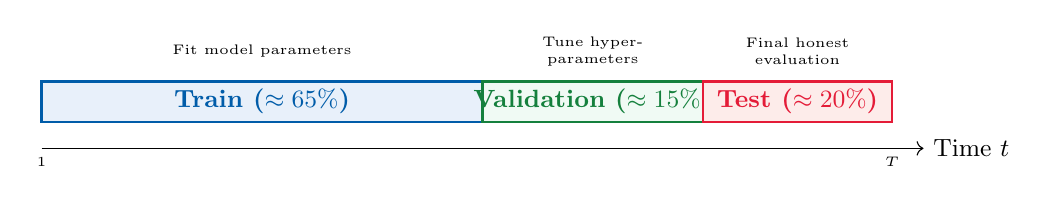
\begin{tikzpicture}[xscale=1.0, yscale=0.85]
    % Train band
    \draw[fill=unolightblue, draw=unoblue, line width=0.8pt]
      (0,0.8) rectangle (5.6, 1.4);
    \node[font=\small\bfseries, color=unoblue] at (2.8, 1.1)
      {Train ($\approx 65\%$)};
    % Validation band
    \draw[fill=unolightgreen, draw=unogreen, line width=0.8pt]
      (5.6,0.8) rectangle (8.4, 1.4);
    \node[font=\small\bfseries, color=unogreen] at (7.0, 1.1)
      {Validation ($\approx 15\%$)};
    % Test band
    \draw[fill=unolightred, draw=unored, line width=0.8pt]
      (8.4,0.8) rectangle (10.8, 1.4);
    \node[font=\small\bfseries, color=unored] at (9.6, 1.1)
      {Test ($\approx 20\%$)};
    % Purpose labels above
    \node[font=\tiny, align=center] at (2.8, 1.85)
      {Fit model parameters};
    \node[font=\tiny, align=center] at (7.0, 1.85)
      {Tune hyper-\\parameters};
    \node[font=\tiny, align=center] at (9.6, 1.85)
      {Final honest\\evaluation};
    % Time arrow
    \draw[->] (0, 0.4) -- (11.2, 0.4)
      node[right, font=\small] {Time $t$};
    \node[font=\tiny] at (0, 0.2) {$1$};
    \node[font=\tiny] at (10.8, 0.2) {$T$};
  \end{tikzpicture}
  \end{center}
  \vspace{-0.05cm}
  \begin{columns}[T]
    \column{0.54\textwidth}
      \textbf{Why three sets, not two?}\\[2pt]
      {\small If you tune on the test set --- even once ---
      it becomes a second validation set, and you no longer have
      an honest generalization estimate.}
    \column{0.42\textwidth}
      \begin{warningbox}
        {\small The test set is a \textbf{time capsule}.
        Open it exactly once, at the very end,
        to report the final number.}
      \end{warningbox}
  \end{columns}
\end{frame}

% --- Slide: Data leakage ------------------------------------------------------
\begin{frame}{Data Leakage: Definition and Examples}
  \begin{definitionbox}{Data Leakage}
    {\small Leakage occurs when information from outside the training
    window contaminates the model, producing optimistic in-sample
    performance that does not generalize out-of-sample.}
  \end{definitionbox}
  \begin{columns}[T]
    \column{0.52\textwidth}
      \textbf{Feature leakage:}
      \begin{itemize}\small
        \item Using next-month CPI to forecast this-month sales
              (future predictor)
        \item Target-encoding computed on the full dataset before
              splitting (statistical leakage)
      \end{itemize}
      \vspace{0.1cm}
      \textbf{Temporal leakage:}
      \begin{itemize}\small
        \item Random train/test shuffle on a time series
        \item Fitting \texttt{StandardScaler} on the full series
              before splitting
      \end{itemize}
    \column{0.44\textwidth}
      \begin{warningbox}
        {\small Random train/test split is \emph{correct}
        for i.i.d.\ data. It is \textbf{wrong} for time
        series. Always split in \textbf{chronological order}.\\[3pt]
        In production: leakage makes reported RMSE
        optimistic by $2\times$--$5\times$.}
      \end{warningbox}
  \end{columns}
\end{frame}

% --- Slide: Time-series-specific rules ----------------------------------------
\begin{frame}{Time-Series Rules for Train/Val/Test}
  \begin{columns}[T]
    \column{0.54\textwidth}
      \begin{enumerate}\small
        \item \textbf{No random shuffling} --- always chronological order
        \item \textbf{Validation after train, test after validation} ---
              strict temporal ordering; no overlaps
        \item \textbf{No future-dependent features} --- any feature using
              time $t+k$ data cannot be known at time $t$
        \item \textbf{Scale within each fold} --- fit
              \texttt{StandardScaler} on train-fold only;
              transform val/test with train parameters
        \item \textbf{Optional gap} --- buffer between train end
              and val start prevents autocorrelation bleed-through
      \end{enumerate}
    \column{0.42\textwidth}
      \begin{keybox}
        {\small These rules are the time-series extensions
        of the bias-variance discipline.\\[3pt]
        Break them and every accuracy number
        you report is invalid.\\[3pt]
        \texttt{train\_test\_split(shuffle=False)}
        respects ordering.
        Use \texttt{TimeSeriesSplit} for CV.}
      \end{keybox}
  \end{columns}
\end{frame}

% =============================================================================
\section{Cross-Validation for Time Series}
% =============================================================================

\sectionslide{Cross-Validation for Time Series}{%
  Standard $k$-fold CV violates time ordering. Walk-forward CV is the fix.}

% --- Slide: Why k-fold is wrong -----------------------------------------------
\begin{frame}{Why $k$-Fold CV is Wrong for Time Series}
  \begin{columns}[T]
    \column{0.50\textwidth}
      \textbf{Standard 5-fold (shuffled):}
      \begin{center}
      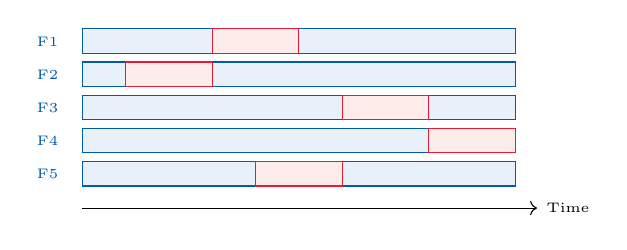
\begin{tikzpicture}[xscale=0.55, yscale=0.7]
        % Show 5 folds with non-chronological test blocks
        % Fold 1: test = middle block (red), rest = blue
        \foreach \y/\teststart/\testend in
          {2.0/3/5, 1.4/1/3, 0.8/6/8, 0.2/8/10, -0.4/4/6} {
          \draw[fill=unolightblue, draw=unoblue, line width=0.4pt]
            (0, \y) rectangle (10, \y+0.45);
          \draw[fill=unolightred, draw=unored, line width=0.4pt]
            (\teststart, \y) rectangle (\testend, \y+0.45);
        }
        \draw[->] (0,-0.8) -- (10.5,-0.8)
          node[right, font=\tiny] {Time};
        \node[font=\tiny, color=unoblue] at (-0.8, 2.22) {F1};
        \node[font=\tiny, color=unoblue] at (-0.8, 1.62) {F2};
        \node[font=\tiny, color=unoblue] at (-0.8, 1.02) {F3};
        \node[font=\tiny, color=unoblue] at (-0.8, 0.42) {F4};
        \node[font=\tiny, color=unoblue] at (-0.8, -0.18) {F5};
      \end{tikzpicture}
      \end{center}
      {\small \negc{Wrong for time series:} validation block
      may precede some training data $\Rightarrow$ temporal leakage.}
    \column{0.46\textwidth}
      \textbf{Failure modes:}
      \begin{itemize}\small
        \item Uses future data to predict the past
        \item Train and validation observations are not
              exchangeable under autocorrelation
        \item Validation RMSE is optimistically biased
      \end{itemize}
      \vspace{0.1cm}
      \begin{warningbox}
        {\small \textcite{Bergmeir2018}: random $k$-fold gives
        biased CV estimates for autoregressive series.
        The bias grows with autocorrelation strength.}
      \end{warningbox}
  \end{columns}
\end{frame}

% --- Slide: Walk-forward CV and TimeSeriesSplit --------------------------------
\begin{frame}[fragile]{Walk-Forward CV and \texttt{TimeSeriesSplit}}
  \textbf{The correct analog:} expanding-window validation introduced in L06,
  now applied to hyperparameter tuning.
  \begin{center}
  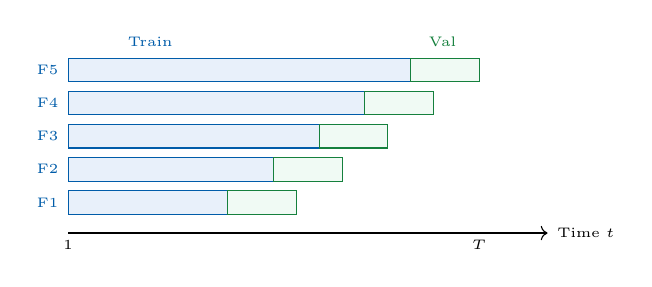
\begin{tikzpicture}[xscale=0.58, yscale=0.60]
    % Fold 1: y = 0.0 to 0.5
    \node[font=\tiny, color=unoblue, left] at (0, 0.25) {F1};
    \draw[fill=unolightblue, draw=unoblue, line width=0.4pt]
      (0,0.0) rectangle (3.5, 0.5);
    \draw[fill=unolightgreen, draw=unogreen, line width=0.4pt]
      (3.5,0.0) rectangle (5.0, 0.5);
    % Fold 2: y = 0.7 to 1.2
    \node[font=\tiny, color=unoblue, left] at (0, 0.95) {F2};
    \draw[fill=unolightblue, draw=unoblue, line width=0.4pt]
      (0,0.7) rectangle (4.5, 1.2);
    \draw[fill=unolightgreen, draw=unogreen, line width=0.4pt]
      (4.5,0.7) rectangle (6.0, 1.2);
    % Fold 3: y = 1.4 to 1.9
    \node[font=\tiny, color=unoblue, left] at (0, 1.65) {F3};
    \draw[fill=unolightblue, draw=unoblue, line width=0.4pt]
      (0,1.4) rectangle (5.5, 1.9);
    \draw[fill=unolightgreen, draw=unogreen, line width=0.4pt]
      (5.5,1.4) rectangle (7.0, 1.9);
    % Fold 4: y = 2.1 to 2.6
    \node[font=\tiny, color=unoblue, left] at (0, 2.35) {F4};
    \draw[fill=unolightblue, draw=unoblue, line width=0.4pt]
      (0,2.1) rectangle (6.5, 2.6);
    \draw[fill=unolightgreen, draw=unogreen, line width=0.4pt]
      (6.5,2.1) rectangle (8.0, 2.6);
    % Fold 5: y = 2.8 to 3.3
    \node[font=\tiny, color=unoblue, left] at (0, 3.05) {F5};
    \draw[fill=unolightblue, draw=unoblue, line width=0.4pt]
      (0,2.8) rectangle (7.5, 3.3);
    \draw[fill=unolightgreen, draw=unogreen, line width=0.4pt]
      (7.5,2.8) rectangle (9.0, 3.3);
    % Time axis
    \draw[->] (0,-0.4) -- (10.5,-0.4)
      node[right, font=\tiny] {Time $t$};
    \node[font=\tiny] at (0,-0.65) {$1$};
    \node[font=\tiny] at (9.0,-0.65) {$T$};
    \node[font=\tiny, color=unoblue] at (1.8, 3.65) {Train};
    \node[font=\tiny, color=unogreen] at (8.2, 3.65) {Val};
  \end{tikzpicture}
  \end{center}
  \vspace{-0.3cm}
  \begin{columns}[T]
    \column{0.52\textwidth}
      {\small
      \begin{lstlisting}[language=Python, basicstyle=\ttfamily\tiny,
                         frame=none, xleftmargin=0pt]
from sklearn.model_selection import TimeSeriesSplit
tscv = TimeSeriesSplit(n_splits=5, gap=0)
for train_idx, val_idx in tscv.split(X):
    X_train, X_val = X[train_idx], X[val_idx]
      \end{lstlisting}
      }
    \column{0.44\textwidth}
      \begin{keybox}
        {\small \texttt{gap}: skip observations between
        train end and val start. Set \texttt{gap=}$H$ when
        forecasting $H$ steps ahead to prevent overlap.}
      \end{keybox}
  \end{columns}
  \muted{\footnotesize\itshape
    General CV theory: \parencite{Arlot2010}.}
\end{frame}

% --- Slide: CV for hyperparameter tuning ---------------------------------------
\begin{frame}{CV in Practice: Hyperparameter Tuning}
  \begin{columns}[T]
    \column{0.52\textwidth}
      \begin{enumerate}\small
        \item Choose candidate values:
              $\lambda \in \{0.01, 0.1, 1, 10, 100\}$
        \item For each $\lambda$: run \texttt{TimeSeriesSplit} CV,
              compute mean validation RMSE
        \item Select $\lambda^*$ minimising mean CV RMSE
        \item \textbf{Refit on full train + val} with $\lambda^*$
        \item Evaluate exactly once on held-out test set
      \end{enumerate}
      \vspace{0.1cm}
      \textbf{Step 4 is critical:} refit on all non-test data.
      Using the CV train-fold only wastes data.
    \column{0.44\textwidth}
      \begin{examplebox}{LASSO on RSXFS}
        {\small 5-fold \texttt{TimeSeriesSplit}:\\[2pt]
        $\lambda=0.1 \Rightarrow$ CV RMSE $= 1{,}780$
        (optimal)\\
        $\lambda=0.001$ (overfit): $1{,}890$\\
        $\lambda=100$ (underfit): $2{,}140$\\[3pt]
        Test RMSE with $\lambda^* = 0.1$: $1{,}620$.}
      \end{examplebox}
  \end{columns}
\end{frame}

% =============================================================================
\section{Regularization Preview}
% =============================================================================

\sectionslide{Regularization Preview}{%
  When there are many predictors, unconstrained OLS overfits.
  Shrinkage is the solution. Full treatment: Lecture~8.}

% --- Slide: Ridge, LASSO, Elastic Net -----------------------------------------
\begin{frame}{Ridge, LASSO, and Elastic Net}
  \begin{definitionbox}{Penalized Regression \parencite{Hastie2009}}
    {\small
    \[
      \hat{\beta} = \arg\min_\beta
      \underbrace{\sum_{t=1}^T (y_t - \beta^\top x_t)^2}_{\text{OLS loss}}
      \;+\; \lambda \cdot P(\beta)
    \]
    \textbf{Ridge:} $P(\beta) = \lVert\beta\rVert_2^2$
    \quad \textbf{LASSO \parencite{Tibshirani1996}:}
    $P(\beta) = \lVert\beta\rVert_1$
    \quad \textbf{EN \parencite{Zou2005}:}
    $\alpha\lVert\beta\rVert_1 + (1{-}\alpha)\lVert\beta\rVert_2^2$
    }
  \end{definitionbox}
  \begin{columns}[T]
    \column{0.54\textwidth}
      \begin{itemize}\small
        \item \textbf{Ridge}: shrinks all coefficients smoothly;
              none reach exactly zero
        \item \textbf{LASSO}: sets some coefficients to exactly
              zero $\Rightarrow$ automatic variable selection
        \item \textbf{Elastic Net}: handles collinear predictors;
              ridge + LASSO combined
      \end{itemize}
    \column{0.42\textwidth}
      \muted{\footnotesize
        All three trade bias for variance via $\lambda$.\\[3pt]
        $\lambda = 0$: OLS (maximum variance).\\
        $\lambda \to \infty$: intercept only (maximum bias).\\[3pt]
        Full derivation in L08.}
  \end{columns}
\end{frame}

% --- Slide: Shrinkage as complexity control ------------------------------------
\begin{frame}{Shrinkage as Complexity Control}
  \begin{columns}[T]
    \column{0.52\textwidth}
      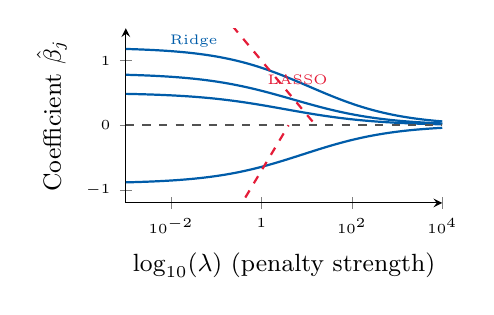
\begin{tikzpicture}
        \begin{axis}[
          width=5.6cm, height=3.8cm,
          xlabel={\small $\log_{10}(\lambda)$ (penalty strength)},
          ylabel={\small Coefficient $\hat{\beta}_j$},
          xmin=-3, xmax=4, ymin=-1.2, ymax=1.5,
          xtick={-2,0,2,4},
          xticklabels={$10^{-2}$, $1$, $10^2$, $10^4$},
          ytick={-1,0,1},
          tick label style={font=\tiny},
          label style={font=\small},
          axis lines=left,
        ]
          % Ridge: smooth curves converging to 0
          \addplot[color=unoblue, thick,
                   domain=-3:4, samples=100]
            { 1.2 / (1 + 0.35*exp(x)) };
          \addplot[color=unoblue, thick,
                   domain=-3:4, samples=100]
            { 0.8 / (1 + 0.5*exp(x)) };
          \addplot[color=unoblue, thick,
                   domain=-3:4, samples=100]
            { -0.9 / (1 + 0.4*exp(x)) };
          \addplot[color=unoblue, thick,
                   domain=-3:4, samples=100]
            { 0.5 / (1 + 0.6*exp(x)) };
          % LASSO: paths reach 0 at different lambda
          \addplot[color=unored, dashed, thick,
                   domain=-3:1.2, samples=100]
            { 1.0 - x/1.2 };
          \addplot[color=unored, dashed, thick,
                   domain=-3:0.6, samples=100]
            { -0.7 + x/(-0.6) * (-0.7) };
          \draw[dashed, color=unogray, line width=0.6pt]
            (axis cs: -3, 0) -- (axis cs: 4, 0);
          \node[font=\tiny, color=unoblue] at (axis cs:-1.5, 1.3)
            {Ridge};
          \node[font=\tiny, color=unored] at (axis cs:0.8, 0.7)
            {LASSO};
        \end{axis}
      \end{tikzpicture}
    \column{0.44\textwidth}
      \begin{keybox}
        {\small As $\lambda \to \infty$:
        $\hat{\beta}_j \to 0$ (all predictors removed).\\[3pt]
        As $\lambda \to 0$: OLS solution.\\[3pt]
        LASSO paths hit zero at a finite $\lambda$ ---
        Ridge paths only approach zero asymptotically.\\[3pt]
        CV selects $\lambda^*$ at the
        bias-variance minimum.}
      \end{keybox}
  \end{columns}
  \muted{\footnotesize\itshape
    Illustrative paths. L08 derives the exact form
    from the subgradient conditions.}
\end{frame}

% =============================================================================
\section{Feature Engineering Preview}
% =============================================================================

\sectionslide{Feature Engineering Preview}{%
  ML models do not handle time series natively.
  We must create temporal structure explicitly.
  Full treatment: Lecture~11.}

% --- Slide: From time series to feature matrix ---------------------------------
\begin{frame}{From Time Series to Feature Matrix}
  A raw series $y_1, \ldots, y_T$ is not a feature matrix.
  We extract temporal patterns as columns.
  \begin{center}
    {\footnotesize
    \begin{tabular}{llp{3.8cm}}
      \toprule
      \textbf{Feature type} & \textbf{Formula} & \textbf{Business meaning} \\
      \midrule
      Lag            & $x_t^{(k)} = y_{t-k}$
                     & Sales $k$ periods ago \\
      Rolling mean   & $\bar{y}_{t,w} = \tfrac{1}{w}\sum_{k=1}^{w} y_{t-k}$
                     & Recent trend level \\
      Rolling std    & $s_{t,w} = \operatorname{std}(y_{t-w:t-1})$
                     & Recent volatility \\
      Month-of-year  & $\mathbf{1}[\operatorname{month}(t) = m]$
                     & Seasonal dummy \\
      Trend counter  & $t = 1, 2, \ldots, T$
                     & Linear time trend \\
      \bottomrule
    \end{tabular}
    }
  \end{center}
  \begin{warningbox}
    {\small All features \textbf{must} use only
    $y_1, \ldots, y_{t-1}$ when predicting $y_t$.
    Any feature using $y_t$ or later creates leakage.
    Apply \texttt{.shift(1)} before any rolling window.}
  \end{warningbox}
  \muted{\footnotesize\itshape
    Full treatment in L11: calendar features, Fourier terms,
    interaction features, and pipeline automation.}
\end{frame}

% --- Slide: Feature engineering in Python ------------------------------------
\begin{frame}[fragile]{Features + Leakage Prevention in Python}
  \begin{columns}[T]
    \column{0.52\textwidth}
      {\small
      \begin{lstlisting}[language=Python, basicstyle=\ttfamily\footnotesize,
                         frame=single, xleftmargin=0pt, framexleftmargin=2pt]
# Lag features: shift(1) avoids leakage
X['lag_1']  = y.shift(1)
X['lag_12'] = y.shift(12)

# Rolling mean of y_{t-1}...y_{t-3}
X['roll_3'] = y.shift(1).rolling(3).mean()

# Calendar feature (always known)
X['month'] = y.index.month

# Drop rows with NaN from lags
X = X.dropna()
      \end{lstlisting}
      }
    \column{0.44\textwidth}
      \begin{itemize}\small
        \item \texttt{.shift(1)}: shifts series forward one
              period --- ensures $x_t$ uses $y_{t-1}$, not $y_t$
        \item \texttt{.rolling(3).mean()} after
              \texttt{.shift(1)}: mean of
              $y_{t-1}, y_{t-2}, y_{t-3}$
        \item \texttt{.index.month}: calendar feature;
              no leakage (calendar is always known in advance)
      \end{itemize}
      \begin{keybox}
        {\small L11 wraps this logic in a
        \texttt{sklearn.Pipeline} that prevents
        leakage automatically at every CV fold.}
      \end{keybox}
  \end{columns}
\end{frame}

% =============================================================================
\section{The ML Forecasting Pipeline}
% =============================================================================

\sectionslide{The ML Forecasting Pipeline}{%
  End-to-end: features $\to$ split $\to$ fit $\to$ evaluate $\to$ deploy.}

% --- Slide: Pipeline architecture ---------------------------------------------
\begin{frame}{The End-to-End ML Forecasting Pipeline}
  \begin{center}
  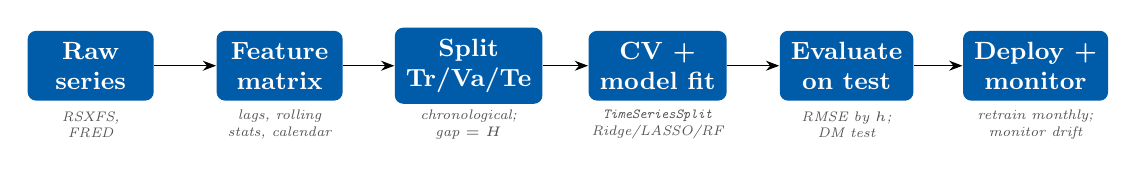
\begin{tikzpicture}[
    box/.style={
      rectangle, rounded corners=3pt,
      fill=unoblue, text=white, align=center,
      minimum width=1.6cm, minimum height=0.7cm,
      font=\small\bfseries, inner sep=4pt
    },
    note/.style={font=\tiny\itshape, color=unogray, align=center},
    >=Stealth
  ]
    \node[box] (raw)   at (0,0)   {Raw\\series};
    \node[box] (feat)  at (2.4,0) {Feature\\matrix};
    \node[box] (split) at (4.8,0) {Split\\Tr/Va/Te};
    \node[box] (fit)   at (7.2,0) {CV +\\model fit};
    \node[box] (eval)  at (9.6,0) {Evaluate\\on test};
    \node[box] (dep)   at (12.0,0){Deploy +\\monitor};

    \draw[->] (raw)   -- (feat);
    \draw[->] (feat)  -- (split);
    \draw[->] (split) -- (fit);
    \draw[->] (fit)   -- (eval);
    \draw[->] (eval)  -- (dep);

    \node[note] at (0,  -0.75) {RSXFS,\\FRED};
    \node[note] at (2.4,-0.75) {lags, rolling\\stats, calendar};
    \node[note] at (4.8,-0.75) {chronological;\\gap $= H$};
    \node[note] at (7.2,-0.75) {\texttt{TimeSeriesSplit}\\Ridge/LASSO/RF};
    \node[note] at (9.6,-0.75) {RMSE by $h$;\\DM test};
    \node[note] at (12.0,-0.75){retrain monthly;\\monitor drift};
  \end{tikzpicture}
  \end{center}
  \vspace{0.0cm}
  \begin{keybox}
    {\small The \texttt{sklearn.Pipeline} object chains preprocessing
    (\texttt{StandardScaler}) + model into a single estimator.
    This ensures the scaler is fitted on train-fold only during CV ---
    eliminating a common source of leakage \parencite{James2021}.}
  \end{keybox}
\end{frame}

% --- Slide: Key takeaways + roadmap -------------------------------------------
\begin{frame}{Key Takeaways and the Road Ahead}
  \begin{columns}[T]
    \column{0.56\textwidth}
      \begin{keybox}
        {\small
        \begin{enumerate}
          \item ML \textbf{extends} classical forecasting for
                non-linearity, many predictors, and unknown structure.
          \item $\MSE = \operatorname{Bias}^2 + \operatorname{Var}
                + \sigma^2$ governs every modelling decision.
          \item Three-way train/val/test split with chronological
                ordering is non-negotiable.
          \item Walk-forward CV (\texttt{TimeSeriesSplit}) replaces
                $k$-fold for time series.
          \item Regularization (L08) and feature engineering (L11)
                are the main levers for controlling bias-variance.
        \end{enumerate}
        }
      \end{keybox}
    \column{0.40\textwidth}
      \textbf{Lecture roadmap:}
      {\footnotesize
      \begin{tabular}{ll}
        \toprule
        \textbf{Lecture} & \textbf{Topic} \\
        \midrule
        L08 & LASSO, Ridge, EN \\
        L09 & RF, XGBoost \\
        L10 & LSTM, attention \\
        L11 & Feature pipeline \\
        L12 & Capstone cases \\
        \bottomrule
      \end{tabular}
      }
      \vspace{0.1cm}
      \muted{\footnotesize\itshape
        Lab 7: full pipeline from raw RSXFS to
        LASSO and Ridge with walk-forward CV.}
  \end{columns}
\end{frame}

% --- References ---------------------------------------------------------------
\begin{frame}[allowframebreaks]{References}
  \printbibliography[heading=none]
\end{frame}

\end{document}
